% ---
% Capa
% ---
\imprimircapa
% ---

% ---
% Folha de rosto
% (o * indica que haverá a ficha catalográfica)
% ---
\imprimirfolhaderosto
% ---

% ---
% Ficha Catalografica em pdf e código
% 
% ---

%\begin{fichacatalografica}
%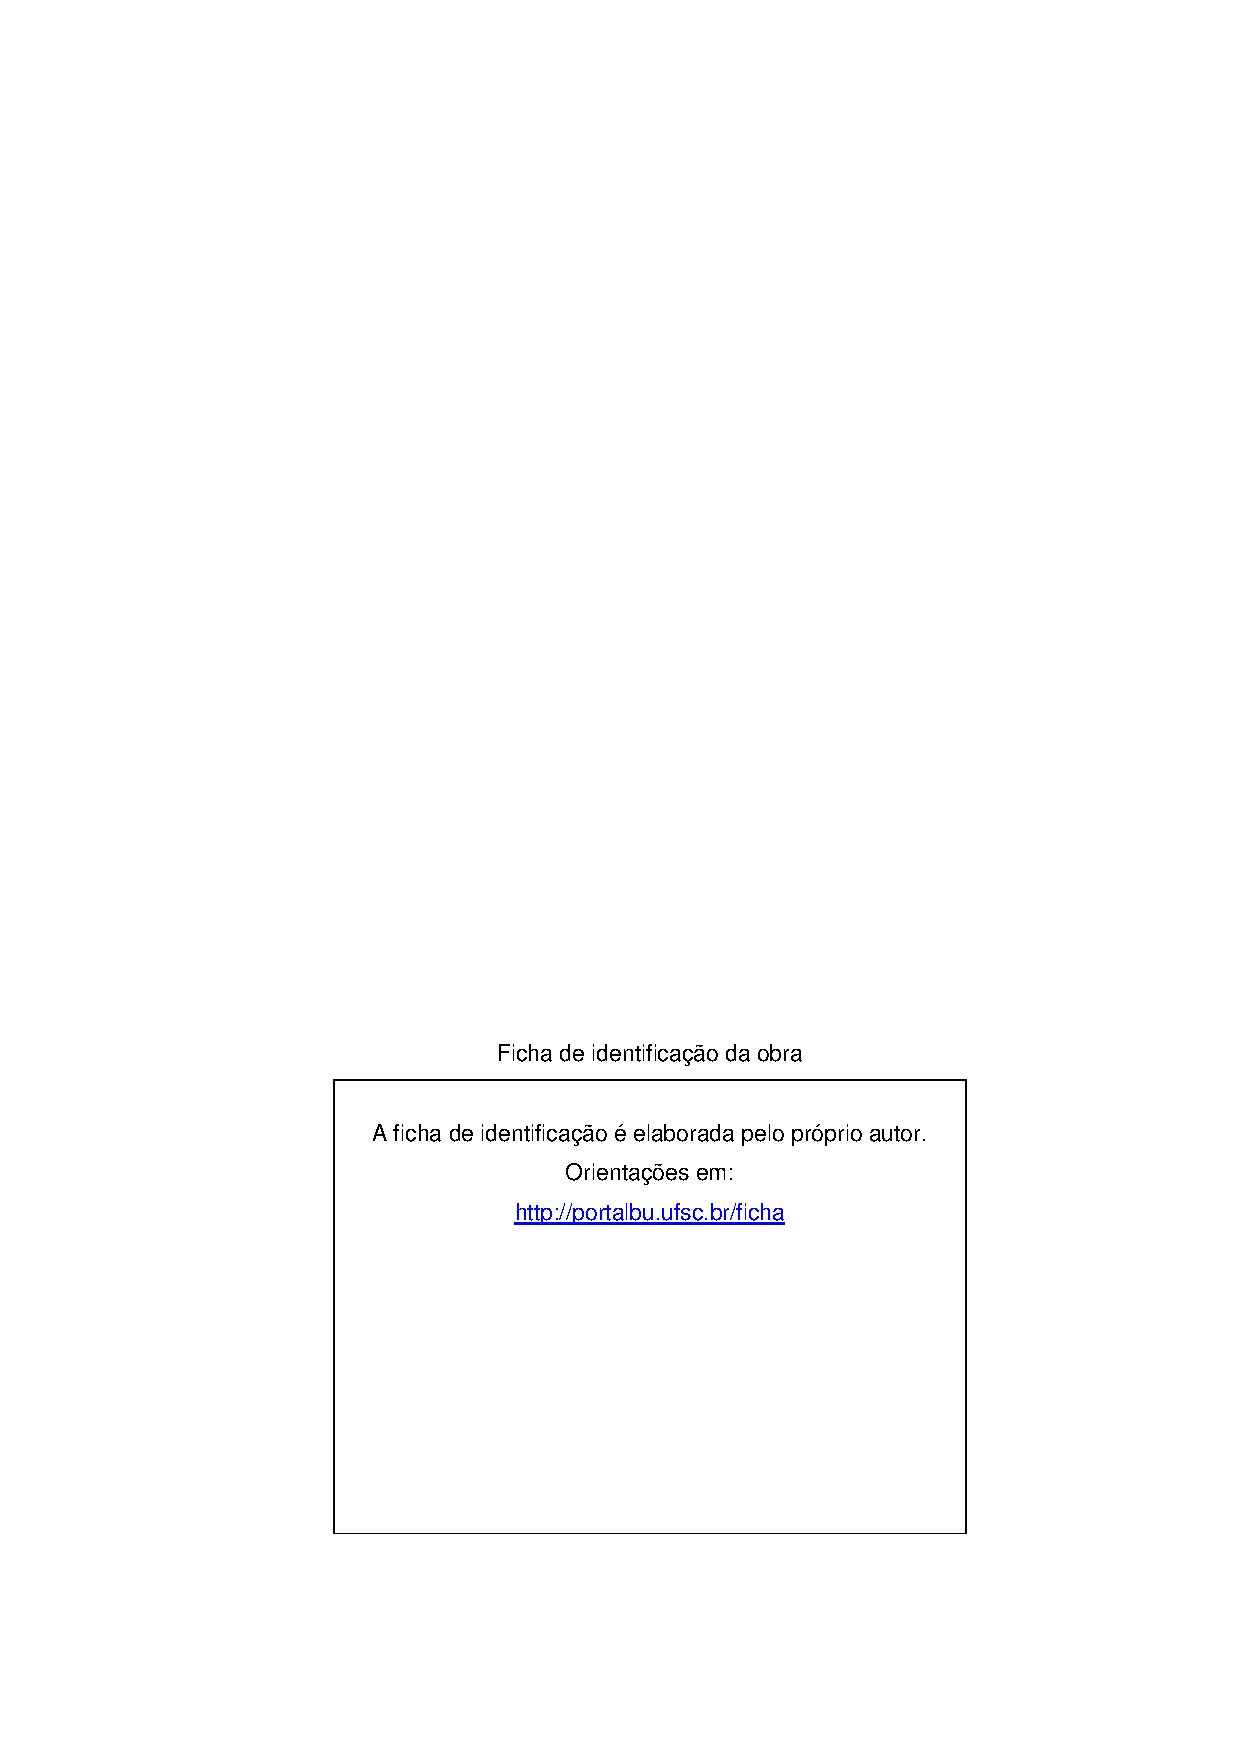
\includepdf{pre/Ficha_Catalografica.pdf}
%\end{fichacatalografica}

%\begin{fichacatalografica}
\vspace*{12cm} % Posição vertical
%\hrule % Linha horizontal

\begin{center} % Minipage Centralizado
\small{\textbf{\cip}}
\framebox[120mm]{%Inicio da caixa
\begin{minipage}{105mm} % Largura [c]{12.5cm}
\begin{flushleft}
\codnome
\end{flushleft}
\imprimirautor

\hspace{0.5cm} \imprimirtitulo / \imprimirautor. --
\imprimirlocal:~\sigla,~\ano.

\hspace{0.5cm} \pageref{LastPage} p. : il.~color.; 30 cm.\\

\hspace{0.5cm} \imprimirorientadorRotulo:~ \imprimirorientador\\

\hspace{0.5cm}
\parbox[t]{\textwidth}{\tcc~--~\imprimirinstituicao,~\campus~--~\curso~\ano.}\\

\hspace{0.5cm}
1. \palavrachaveum.
2. \palavrachavedois.
3. \palavrachavetres.
4. \palavrachavequatro.
5. \palavrachavecinco.
I. \MakeUppercase{\sobrenomeorient},~\nomeorient~\sigorient..
%II. Universidade xxx.
%III. Faculdade de xxx.
II. T\'tulo.\\

%\hspace{7.75cm} \cdu\\
\begin{flushright}
    						\cdu
\end{flushright}%
%\hspace{8.75cm}
\end{minipage}
}%Fim caixa
\par
\vspace{0.1cm}
Ficha catalogr\'afica elaborada pelo bibliotec\'ario~\bibliotecario~\cbr
\par
Biblioteca Clarice Lispector
\par
\imprimirinstituicao
\par
Campus: An\'apolis

\end{center}

%\hrule
\end{fichacatalografica}

%----------------------------------------------


% ---
% Inserir folha de aprovação
% ---
%\begin{folhadeaprovacao}
	\OnehalfSpacing
	\centering
	\imprimirautor\\%
	\vspace*{10pt}		
	\textbf{\imprimirtitulo}%
	\ifnotempty{\imprimirsubtitulo}{~\imprimirsubtitulo}\\%
	%		\vspace*{31.5pt}%3\baselineskip
	\vspace*{\baselineskip}
	%\begin{minipage}{\textwidth}
	% ~do~\imprimirprograma~do~\imprimircentro~da~\imprimirinstituicao~para~a~obtencao~do~título~de~\imprimirformacao.
	Este~\imprimirtipotrabalho~foi julgado adequado para obten\c{c}\~ao do T\'itulo de ''\imprimirformacao'' e aprovado em sua forma final pelo~\imprimirprograma. \\
		\vspace*{\baselineskip}
	\imprimirlocal, \imprimirdata. \\
	\vspace*{2\baselineskip}
	\assinatura{\OnehalfSpacing\imprimircoordenador \\ \imprimircoordenadorRotulo~do Curso}
	\vspace*{2\baselineskip}
	\textbf{Banca Examinadora:} \\
	\vspace*{\baselineskip}
	\assinatura{\OnehalfSpacing\imprimirorientador \\ \imprimirorientadorRotulo}
	%\end{minipage}%
	\vspace*{\baselineskip}
	\assinatura{Prof.(a) xxxx, Dr(a).\\
	Avaliador(a) \\
	Institui\c{c}\~ao xxxx}

	\vspace*{\baselineskip}
	\assinatura{Prof.(a) xxxx, Dr(a).\\
	Avaliador(a) \\
	Institui\c{c}\~ao xxxx}


\end{folhadeaprovacao}
% ---

% ---
% Inserir folha de ata da seção pública de tcc
% ---
%\linespread{0.87}

%--------Cabeçalho do documento
\noindent\begin{minipage}[c][1.5cm][c]{3.5cm}
%\includegraphics[height=1.5cm]{./figuras/logoEvangelica.eps}

\includegraphics[width=1.5 \textwidth]{./outros/fig/IFGAnapolisHor2.png}
\end{minipage}\quad\quad\quad\qquad
\begin{minipage}{12cm}%10cm
\scriptsize\textbf{\ministerio}\\%\sc
\textbf{\secretaria}\\
\textbf{\instituto}\\
\textbf{\reitoria}\\
\end{minipage}
\vspace{1cm}
%---------------------------------------------------------------------------------------


\begin{center}
	\textbf{ATA N\textsuperscript{o} 20/2022.1}\\
	\footnotesize{\MakeUppercase{\textbf{Ata da sess\~ao p\'ublica de apresenta\c{c}\~ao do trabalho de conclus\~ao de curso 2}}}
\end{center}
\vspace{1.0cm}
\noindent Aos~0\diaata~dias do m\^es de~\mesata~do ano de dois mil e vinte dois, \'as~\hinicial~horas, por meio de webconfer\^encia utilizando Google Meet, foi realizada a sess\~ao p\'ublica de apresenta\c{c}\~ao do Trabalho de Conclus\~ao 2 da Graduando~\textbf{\alunonome~\alunosobre}~(matr\'icula~\matricula) do curso de~\curso. A banca foi composta pelos seguintes membros:~\orientadora,~\membroum,~\membrodois, sob a presid\^encia da primeira. O trabalho de conclus\~ao de curso tem como t\'itulo ``\textbf{\titulo}'', da \'area de Geotecnia, sob orienta\c{c}\~ao da Prof\textsuperscript{a}~\orientadora. Ap\'os a apresenta\c{c}\~ao do Trabalho de Conclus\~ao de Curso 2, tendo sido o autor arguido pela Banca Examinadora, a nota obtida foi~\notanumerico~(\notaextenso).
\\
\\
\noindent Encerra-se a presente sess\~ao \'as~\hfinal~horas~e~\mfinal~minutos. Eu Prof\textsuperscript{a}.~\orientadora, dato e assino a presente ata que segue assinada por todos os membros da Banca e pelo graduando.
\vspace{1.0cm}
\small{
\begin{center}
\begin{tabular}{c}
\multicolumn{1}{c}{\asseletronica} \\ 
\multicolumn{1}{c}{Prof\textsuperscript{a}~\orientadora} \\ 
\multicolumn{1}{c}{} \\ 
\asseletronica \\ 
\multicolumn{1}{c}{Prof\textsuperscript{a}~\membroum~} \\ 
\multicolumn{1}{c}{~} \\ 
\asseletronica\\
%
\includegraphics[width=0.30 \textwidth]{./outros/fig/AssDaniel.jpg} \\ %\hrulefill comando para linha
\multicolumn{1}{c}{Prof\textsuperscript{a}~\membrodois~} \\ 
\multicolumn{1}{c}{~} \\ 
\includegraphics[width=0.25 \textwidth]{./outros/fig/minhaAssinatura.png} \\
\multicolumn{1}{c}{\textbf{\alunonome~\alunosobre}} \\
\multicolumn{1}{c}{(Graduando)} \\
\multicolumn{1}{c}{~} \\ 
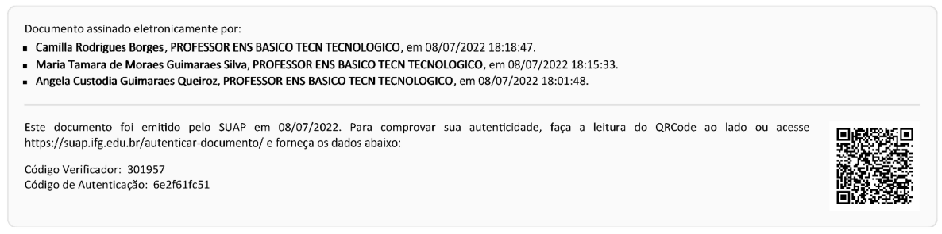
\includegraphics[width=0.97 \textwidth]{./outros/fig/QR_CODE_V2.pdf}
\\
\end{tabular}
\end{center}
}

\linespread{1.3}
\newpage





% ---
% Inserir folha de autorização para disponibilização
% ---
%\linespread{0.87}
%--------Cabeçalho do documento
\noindent\begin{minipage}[c][1.5cm][c]{3.5cm}

\includegraphics[width=1.5 \textwidth]{./outros/fig/IFGAnapolisHor2.png}
\end{minipage}\quad\quad\quad\qquad
\begin{minipage}{12cm}%10cm
\scriptsize\textbf{\ministerio}\\
\textbf{\secretaria}\\
\textbf{\instituto}\\
\textbf{\MakeTextUppercase{\campus}}\\
\textbf{\biblioteca}\\
\end{minipage}
%\vspace{-0.1cm}
\small{
\begin{center}
	\termo
\end{center}

%Com base do disposto na Lei Federal nº 9.610/98, AUTORIZO o~\entidade, a disponibilizar gratuitamente o documento no Reposit\'orio Digital (ReDi~\sigla), sem ressarcimento de direitos autorais, conforme permiss\~ao assinada abaixo, em formato digital para fins de leitura, download e impress\~ao, a t\'itulo de divulga\c{c}\~ao de produ\c{c}\~ao t\'ecnico-cient\'ifica no IFG.
\termodois

\noindent \textbf{Identifica\c{c}\~ao de Produ\c{c}\~ao T\'ecnico-Cient\'ifica}

\begin{tabular}{lllll}
\lbrack ~~\rbrack & Tese &  & \lbrack ~~\rbrack & Artigo Cient\'ifico \\ 
\lbrack ~~\rbrack & Disserta\c{c}\~ao &  & \lbrack ~~\rbrack & Cap\'itulo de Livro \\ 
\lbrack ~~\rbrack & Monografia -- Especializa\c{c}\~ao &  & \lbrack ~~\rbrack & Livro \\ 
\lbrack X\rbrack & TCC -- Gradua\c{c}\~ao &  & \lbrack ~~\rbrack & Trabalho Apresentado em Evento \\ 
\lbrack ~~\rbrack & Produto T\'ecnico e Educacional -- Tipo: & \multicolumn{3}{l}{\hrulefill} \\ 
\end{tabular}

\quad

\noindent Nome Completo do Autor:~\textbf{\alunonome~\alunosobre}

\noindent Matr\'icula:~\textbf{\matricula}

\noindent T\'ituto do Trabalho:~\textbf{\tituloprincipal}

\noindent \textbf{Autoriza\c{c}\~ao -- Marque uma das op\c{c}\~oes}

\begin{enumerate}
	\item (X) Autorizo disponibilizar meu trabalho no Reposit\'orio Digital do IFG (acesso aberto);
	\item (~) Autorizo disponibilizar meu trabalho no Reposit\'orio Digital do IFG somente ap\'os a data 20/10/20 (Embargo);
	\item (~) N\~ao autorizo disponibilizar meu trabalho no Reposit\'orio Digital do IFG (acesso restrito)
\end{enumerate}

\noindent Ao indicar a op\c{c}\~ao \textbf{2 ou 3}, marque a justificativa:
\begin{description}
	\item[(~~)] O documento est\'a sujeito a registro de patente.
	\item[(~~)] O documento pode vir a ser publicado como livro, cap\'itulo de livro ou artigo.
	\item[(~~)] Outra justificativa: \hrulefill
\end{description}

\begin{center}
	\textbf{\declaracao}
\end{center}

\noindent O(A) referido(a) autor(a) declara que:

\textbf{(i)}~o documento \'e seu trabalho original, det\'em os direitos autorais de produ\c{c}\~ao t\'ecnico-cient\'ifica e n\~ao infringe os direitos de qualquer outro pessoa ou entidade;

\textbf{(ii)}~\termotres

\textbf{(iii)}~cumpriu quaisquer obriga\c{c}\~oes exigidas por contrato ou acordo, caso o documento entregue seja baseado em trabalho finaciado ou apoiado por outra institui\c{c}\~ao que n\~ao o \entidade.

%\todaydia
\begin{flushright}
An\'apolis, {\diaata~de~\mesata}~de~{\todayano}
\end{flushright}

\begin{center}
\begin{tabular}{c}
\includegraphics[width=0.19 \textwidth]{./outros/fig/minhaAssinatura.png} \\ 
\multicolumn{1}{c}{~\alunonome \alunosobre} \\ 
%\multicolumn{1}{c}{\hrulefill} \\ 
\end{tabular}
\end{center}
}%Fim \small

\linespread{1.3}

\newpage

%\begin{figure}[htbp]
%	\centering
%		\includegraphics[width=0.30 %\textwidth]{./outros/fig/minhaAssinatura.png}%
%	\label{fig:minhaAssinatura}
%\end{figure}


%\begin{minipage}{12cm}
%\begin{tabular}{p{12cm}}
%\textbf{\scriptsize{\uppercase{Minist\'erio da Educa\c{c}\~ao}}}\\
%\textbf{\scriptsize{\uppercase{Secretaria de Educa\c{c}\~ao Profissional e Tecnol\'ogica}}}\\
%\textbf{\scriptsize{\uppercase{Instituto Federal de Educa\c{c}\~ao, Ci\^encia e Tecnologia}}}\\
%\textbf{\scriptsize{\uppercase{Pr\'o-reitoria de Pesquisa e P\'os-Gradua\c{c}\~ao}}} \\
%\textbf{\scriptsize{\uppercase{Sistema Integrado de Bibliotecas}}} \\  
%\end{tabular}
%\end{minipage}

%\begin{minipage}{12cm}%10cm
%\scriptsize\textbf{\ministerio}\\
%\textbf{\secretaria}\\
%\textbf{\instituto}\\
%\textbf{\campus}\\
%\textbf{\biblioteca}\\
%\end{minipage}




% ---
% Dedicatória
% ---
%\begin{dedicatoria}
%	\vspace*{\fill}
%	\noindent
%	\begin{adjustwidth*}{}{5.5cm}     
%		Este trabalho é dedicado aos meus colegas de classe e aos meus queridos pais.
%	\end{adjustwidth*}
%\end{dedicatoria}
% ---

% ---
% Agradecimentos
% ---
%\begin{agradecimentos}
%	Inserir os agradecimentos aos colaboradores à execução do trabalho. 
	
	%Xxxxxxxxxxxxxxxxxxxxxxxxxxxxxxxxxxxxxxxxxxxxxxxxxxxxxxxxxxxxxxxxxxxxxx. 
%\end{agradecimentos}
% ---

% ---
% Epígrafe
% ---
%\begin{epigrafe}
%\vspace*{\fill}
	%'\begin{flushright}
		%'\textit{%''Texto da Epígrafe.\\
			%Citação relativa ao tema do trabalho.\\
		%É opcional. A epígrafe pode também aparecer\\
			%na abertura de cada seção ou capítulo.\\
			%Deve ser elaborada de acordo com a NBR 10520.''\\
			%(Autor da epígrafe, ano)
	%''Não se gerencia o que não se mede,\\
	%não se mede o que não se define,\\
	%não se define o que não se entende,\\
	%e não há sucesso no que não se gerencia''\\
	%(William Edwards Deming)
%}
%	\end{flushright}
%\end{epigrafe}
% ---

% ---
% RESUMOS
% ---

% resumo em português
%\setlength{\absparsep}{18pt} % ajusta o espaçamento dos parágrafos do resumo
%\begin{resumo}
%	\SingleSpacing
%	No resumo são ressaltados o objetivo da pesquisa, o método utilizado, as discussões e os resultados com destaque apenas para os pontos principais. O resumo deve ser significativo, composto de uma sequência de frases concisas, afirmativas, e não de uma enumeração de tópicos. Não deve conter citações. Deve usar o verbo na voz ativa e na terceira pessoa do singular. O texto do resumo deve ser digitado, em um único bloco, sem espaço de parágrafo. O espaçamento entre linhas é simples e o tamanho da fonte é 12. Abaixo do resumo, informar as palavras-chave (palavras ou expressões significativas retiradas do texto) ou, termos retirados de thesaurus da área. Deve conter de 150 a 500 palavras. O resumo é elaborado de acordo com a NBR 6028.
	
%	\textbf{Palavras-chave}: Palavra-chave 1. Palavra-chave 2. Palavra-chave 3.
%\end{resumo}

% resumo em inglês
%\begin{resumo}[Abstract]
%	\SingleSpacing
%	\begin{otherlanguage*}{english}
%		Resumo traduzido para outros idiomas, neste caso, inglês. Segue o formato do resumo feito na língua vernácula. As palavras-chave traduzidas, versão em língua estrangeira, são colocadas abaixo do texto precedidas pela expressão “Keywords”, separadas por ponto.
		
%		\textbf{Keywords}: Keyword 1. Keyword 2. Keyword 3.
%	\end{otherlanguage*}
%\end{resumo}

%% resumo em francês 
%\begin{resumo}[Résumé]
% \begin{otherlanguage*}{french}
%    Il s'agit d'un résumé en français.
% 
%   \textbf{Mots-clés}: latex. abntex. publication de textes.
% \end{otherlanguage*}
%\end{resumo}
%
%% resumo em espanhol
%\begin{resumo}[Resumen]
% \begin{otherlanguage*}{spanish}
%   Este es el resumen en español.
%  
%   \textbf{Palabras clave}: latex. abntex. publicación de textos.
% \end{otherlanguage*}
%\end{resumo}
%% ---

{%hidelinks
	\hypersetup{hidelinks}
	% ---
	% inserir lista de ilustrações
	% ---
	%\pdfbookmark[0]{\listfigurename}{lof}
	%\listoffigures*
	%\cleardoublepage
	% ---
	
	% ---
	% inserir lista de quadros
	% ---
	%\pdfbookmark[0]{\listofquadrosname}{loq}
	%\listofquadros*
	%\cleardoublepage
	% ---
	
	% ---
	% inserir lista de tabelas
	% ---
	%\pdfbookmark[0]{\listtablename}{lot}
	%\listoftables*
	%\cleardoublepage
	% ---
	
	% ---
	% inserir lista de abreviaturas e siglas (devem ser declarados no preambulo)
	% ---
	%\imprimirlistadesiglas
	% ---
	
	% ---
	% inserir lista de símbolos (devem ser declarados no preambulo)
	% ---
	%\imprimirlistadesimbolos
	% ---
	
	% ---
	% inserir o sumario
	% ---
	\pdfbookmark[0]{\contentsname}{toc}
	\tableofcontents*
	\cleardoublepage
	
}%hidelinks
% ---